\documentclass[dvipdfmx]{jarticle}
\usepackage{amsmath,amssymb}
\usepackage{xfp}
\usepackage[dvipdfmx]{graphicx}


\begin{document}

\title{木製スピニングリールの構造概要設計}
\maketitle

\section{リール全体構造と部位ID}
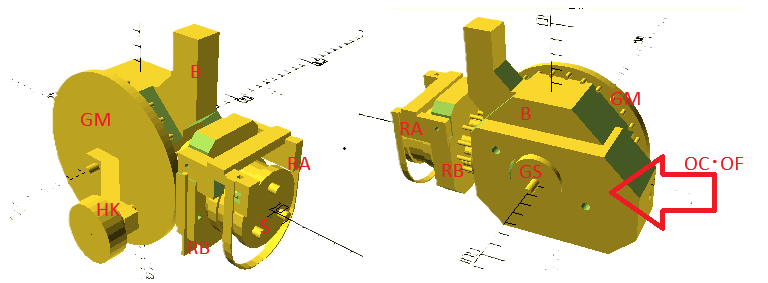
\includegraphics[scale=0.5]{fig/TOTALX.png}
\begin{itemize}
  \item \textbf{[B] ボディ} フット一体 
  \item \textbf{[S] スプール} メインシャフトに沿って前後動, オシレーション機構によって動く
  \item \textbf{[R] ローター} 前後積層構造 / メインシャフトを軸に回転 , ハンドル系によって動く
    \begin{itemize}
      \item \textbf{[RB]} ローターボディ（ピンラックホイールと一体化してアームを保持する, 重要部品の一つ. 前後積層構造）
      \item \textbf{[RA]} アーム（ローターボディ上で可動して糸の巻取り・放出を切り替える部位）
      \item \textbf{[RS]} ストッパー（巻取り時アームを固定する部位）
    \end{itemize}
  \item \textbf{[M] メインシャフト} スプールとローターをボディに保持
  \item \textbf{[H] ハンドル系} 力の入力と伝達, ローターとオシレーション機構を駆動
    \begin{itemize}
      \item \textbf{[HK]} ハンドル（実際回すところ，ハンドルシャフトに拘束）
      \item \textbf{[HS]} ハンドルシャフト
      \item \textbf{[GM]} メイン冠状歯車（ローターに回転を伝える部位, 歯の位置精度は極めて重要, ハンドルに拘束）
      \item \textbf{[GS]} サブ冠状歯車（オシレーション機構に回転を伝える部位，ハンドルシャフトに拘束）
    \end{itemize}
  \item \textbf{[O] オシレーション機構} ハンドルから受けた回転を前後運動に変換してスプールを駆動
    \begin{itemize}
      \item \textbf{[OC]} カム歯車（ハンドルシャフトから回転を受けるパーツとオシレーション運動を生成するカムが一体になったもの）
      \item \textbf{[OF]} 受け子（カムから力を受けてオシレーションするパーツ, オシレーションシャフトを拘束）
      \item \textbf{[OS]} オシレーションシャフト（オシレーション運動をスプールに伝達するパーツ, 受け子とスプールに拘束）
    \end{itemize}
\end{itemize}
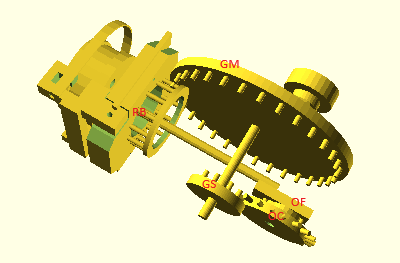
\includegraphics[scale=0.5]{fig/SKELETONX.png}

\section{各パーツの局所的構成（ローカル詳細）}

\subsection*{[B] ボディ詳細}
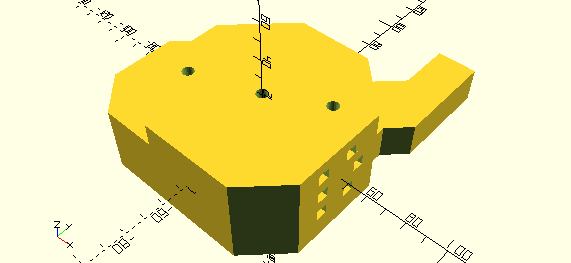
\includegraphics[scale=0.5]{fig/B.png}

各動体機構の受け軸間の位置精度は最も重要
6㎜厚の板で左右積層構造.
 L3-1CR1-3は固着して一体化. L4層は分離可能に.
      \begin{itemize}
        \item \textbf{[B-C]} C層（オシレーションシャフト, フット）
        \item \textbf{[B-L1]} L1層（受け子, フット）
        \item \textbf{[B-L2]} L2層（カム歯車カム部）
        \item \textbf{[B-L3]} L3層（カム歯車歯車部、サブ冠状歯車歯部）
        \item \textbf{[B-L4]} L4層（カム歯車軸受け、サブ冠状歯車基部、ハンドルシャフト左側受け）
		この層のみ一体化せず開けるようにする事でオシレーション機構にアクセスできるようにする
        \item \textbf{[B-R1]} R1層（構造体, フット）
        \item \textbf{[B-R2]} R2層（構造体）
        \item \textbf{[B-R3]} R3層（構造体）ンドルシャフト右側受け, 
		現設計ではメインギアとの間に 3mm分の隙間があり，ワッシャー的な間隔調整部品ががいる
        \item \textbf{[B-F]} フット部分 
      \end{itemize}


フット部分は複雑な機構は一切ないが単純に最も力がかかるという測面で留意が必要.
(魚との力というより人間が巻くときの力が最も大きい. ギア比から言っても当然であるが)


\subsection*{[M] メインシャフト詳細}
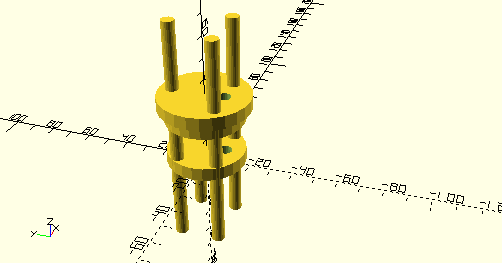
\includegraphics[scale=0.5]{fig/MS.png}

回転するローターの先でスプールが前後する機構上, 一種の中空構造が必須となる.
パイプ状は加工難度が高くなるため, 
ローターの(大)円孔を内接する多角形の頂点で保持する.

6角形の頂点に軸を配置して大円を構成する構造、
ただし6時方向軸はオシレーションシャフトとの干渉を避けるためオミット.
(理論上は三角形の頂点で十分なので)


      \begin{itemize}
        \item \textbf{[M-S0]} S0 (長い, ローターとスプール保持)
        \item \textbf{[M-S2]} S2 (短い, ローター保持)
        \item \textbf{[M-S4]} S4 (長い, ローターとスプール保持)
        \item \textbf{[M-S8]} S8 (長い, ローターとスプール保持)
        \item \textbf{[M-S10]} S10 (短い, ローター保持)
        \item \textbf{[M-Bb]} Bb（シャフトをつなぐ橋構造ボディ側）
        \item \textbf{[M-Bt0]} Bt0（シャフトをつなぐ橋構造トップ側）
        \item \textbf{[M-Bt1]} Bt1（シャフトをつなぐ橋構造トップ側、ローターを保持）
      \end{itemize}

\subsection*{[R] ローター詳細}
		動機構が多く, また魚との間の力を直接受ける部位.
		その割にあまり大きくできないので最も難度の高い部位.
    \begin{itemize}
      \item \textbf{[RB] ローターボディ}
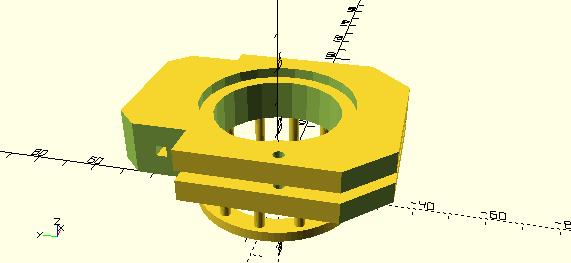
\includegraphics[scale=0.5]{fig/RB.png}
		3㎜厚の板で前後積層構造.
      \begin{itemize}
        \item \textbf{[RB-b]} ピンラックホイールボディ側受け(ピンホイール精度は極めて重要), メインシャフト大円(この円精度は極めて重要)
        \item \textbf{[RB-t0]} ピンラックホイールトップ側受け, メインシャフト大円
        \item \textbf{[RB-t1]} ストッパー、アーム軸, メインシャフト大円
        \item \textbf{[RB-t2]} ストッパーとアーム軸の保持, メインシャフト大円、メインシャフト保持部の受け
        \item \textbf{[RB-t3]} メインシャフト大円、メインシャフト保持部の受け
      \end{itemize}
      \item \textbf{[RA]アーム}
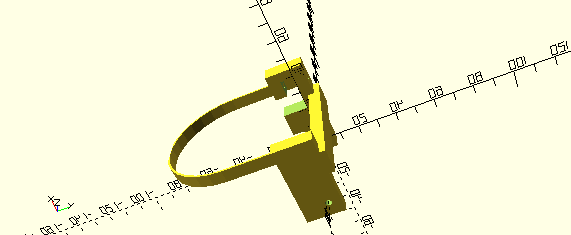
\includegraphics[scale=0.5]{fig/RA.png}

	魚との間の力を初めに受ける部位, その上可動部位で小さい.
	可動のスムーズさは使用感に大きく影響する.
	使用感上, スムーズな巻取りというよりも糸と接触部の摩擦からの保護のためにラインローラー(もどき)は欲しい.
	大きな力を受けたときに逃がす目的なのでローラー自体のスムーズさはほとんどなくても役に立つ.
	細部構造は設計図に反映しきってない(あまり他と干渉しないので後で作りこめる.そう木製ならね)
      \item \textbf{[RS]ストッパー}
	巻取り時にアームの可動を止める部位. 
	使用感に大きく影響する.
	全木製にこだわった時のストッパーのバネは現物合わせで竹をいい感じに削る以上のことが言えない
    \end{itemize}

\subsection*{[H] ハンドル系}
    \begin{itemize}
      \item \textbf{[GM]} メイン冠状歯車
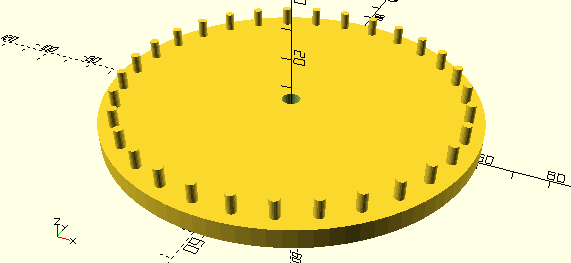
\includegraphics[scale=0.5]{fig/GM.png}
（ローターに回転を伝える部位, 歯の位置精度は極めて重要, ハンドルに拘束）
      \item \textbf{[GS]} サブ冠状歯車
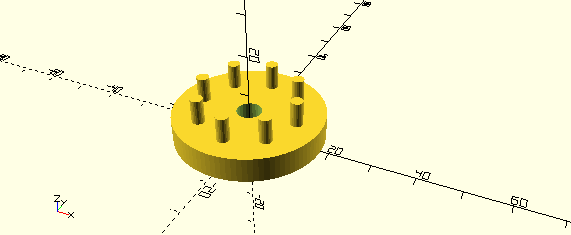
\includegraphics[scale=0.5]{fig/GS.png}
（オシレーション機構に回転を伝える部位，ハンドルシャフトに拘束）
    \end{itemize}

\subsection*{[O] オシレーション機構詳細}
    \begin{itemize}
      \item \textbf{[OC] カム歯車}
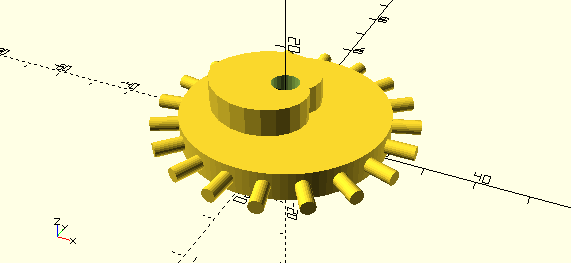
\includegraphics[scale=0.5]{fig/OC.png}
	小型化は要求されるが, 魚との力は直接加わらない上に, 前後のカムの形状精度もそれほど重要ではない.
	(実際問題ハートカムでなく単純な円状カムでオシレーションを正弦波にしても使えなくはない)
      \begin{itemize}
        \item \textbf{[OC-G]} OC-G (歯車)
        \item \textbf{[OC-C]} OC-C (ハートカム)
      \end{itemize}
      \item \textbf{[OF]} 受け子
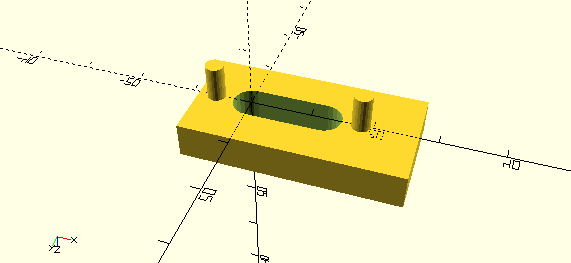
\includegraphics[scale=0.5]{fig/OF.png}
（カムから力を受けてオシレーションするパーツ, オシレーションシャフトを拘束）
      \item \textbf{[OS]} オシレーションシャフト（オシレーション運動をスプールに伝達するパーツ, 受け子とスプールに拘束）
    \end{itemize}

\subsection*{[S] スプール詳細}
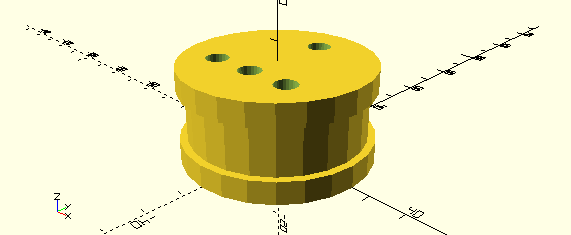
\includegraphics[scale=0.5]{fig/S.png}

	オシレーションの運動方向は魚とかかる力と直交しているので機構に直接力がかかららない.
	また, 円形状は糸の放出のスムーズさにかかわるだけで巻取り機構にはほぼ影響しない(何なら多角形でもあまり問題ない).
	という理由から実は割と適当でいい部品.


\section{機械機構設計}

基体に穴をあけて竹串を指すという形式のピン歯車を基本とする.

形状精度や位置精度や剛性について手加工木製品であるという制限がある中で, 
求められる加工は正確な穴位置だけという破格の工作コストで機能する機構を構成できる. 


一方で工作精度の限界による軸ブレや素材の剛性によるしなり,
手加工故の歯数の少なさから単純な直径比と歯数比以上に駆動被駆動を考慮した歯車が必要となる.


既成の機械機構に比較にならないぐらいのガタツキが出るが, 
それでも工作コストに対するコスパという点では著しいものがある.


\newcounter{GMnum}
\setcounter{GMnum}{31}

\newcounter{GMr}
\setcounter{GMr}{55}

\newcounter{RBnum}
\setcounter{RBnum}{12}

\newcounter{RBr}
\setcounter{RBr}{21}

\newcounter{GSnum}
\setcounter{GSnum}{8}

\newcounter{OCnum}
\setcounter{OCnum}{19}

\newcounter{GSr}
\setcounter{GSr}{12}

\newcounter{OCGSx}
\setcounter{OCGSx}{35}
\newcounter{OCGSy}
\setcounter{OCGSy}{12}


\subsection*{巻取り系}
ハンドル回転から直交する軸ローター回転.
最も力がかかる機構.
加速.



\begin{tabular}{c||c|c}
& [GM]駆動 & [RB]被駆動 \\ \hline
形状& 冠状ピン歯車 & ピンラックホイール \\
基準半径 & \arabic{GMr} mm & \arabic{RBr} mm \\
歯数 & \arabic{GMnum} & \arabic{RBnum} \\
歯間直線距離&
	$\fpeval{2*round( sind( 180/\value{GMnum} ) *\value{GMr}, 1)}$ &
	$\fpeval{2*round( sind( 180/\value{RBnum} ) *\value{RBr}, 1)}$
\end{tabular}

歯間直線距離について
\begin{eqnarray*}
\text{駆動車の歯間直線距離} &\ge& \text{被駆動車の歯間直線距離}\\
\text{ピン直径}\times 2 &\le& \text{歯間直線距離}
\end{eqnarray*}
を満たさなければロックする.
一方で接触歯が次に移るタイミングでほぼ上式差分空転する.

\subsection*{オシレーション系}
凡そ$\fpeval{round(\value{GMnum}*\value{OCnum}/(\value{RBnum}*\value{GSnum}), 1)}$巻きに一周期分オシレートする

\subsubsection*{オシレーション減速径}
ハンドル回転から平行軸カム歯車回転.
減速.

\begin{tabular}{c||c|c}
& [GS]駆動 & [OC]被駆動 \\ \hline
形状& 冠状ピン歯車 & 放射状ピン歯車 \\
基準半径 & \arabic{GSr} mm & - (軸間 $\sqrt{\arabic{OCGSx}^2+\arabic{OCGSy}^2} \doteqdot \fpeval{round(sqrt(\value{OCGSx}*\value{OCGSx}+\value{OCGSy}*\value{OCGSy}), 2)}$ mm ) \\
歯数 & \arabic{GSnum} & \arabic{OCnum} \\
歯間直線距離&
	$\fpeval{2*round( sind( 180/\value{GSnum} ) *\value{GSr}, 1)}$ &
	$\fpeval{2*round( sind( 180/\value{OCnum} ) *(sqrt(\value{OCGSx}*\value{OCGSx}+\value{OCGSy}*\value{OCGSy})-\value{GSr}), 1)}$
\end{tabular}


\subsubsection*{オシレーション系}

\begin{tabular}{c||c|c}
& [OC]駆動 & [OF]被駆動 \\ \hline
形状& 三角波一周期ハートカム & 両端押え \\
基準半径 & 6 mm --- 18 mm &   \\
\end{tabular}





\end{document}




